\documentclass[12pt]{article}
\usepackage[top=1.5cm,bottom=1.5cm,right=2.5cm,left=2.5cm]{geometry}
\usepackage[francais]{babel}
\usepackage[utf8]{inputenc}
\usepackage[T1]{fontenc}
\usepackage[absolute]{textpos} 
\usepackage{graphicx}
\usepackage{caption}
\usepackage{amsthm}

\title{Raja - Bases de données distribuées}

\begin{document}
\vspace{10mm}
\def\blurb{%
   Université des Sciences de Montpellier \\
  Master 2 Semestre 1 \\
  Unité d'Enseignement FMIN306
	}
\def\clap#1{\hbox to 0pt{\hss #1\hss}}%
\def\ligne#1{%
  \hbox to \hsize{%
    \vbox{\centering #1}}}%
\def\haut#1#2#3{%
  \hbox to \hsize{%
    \rlap{\vtop{\raggedright #1}}%
    \hss
    \clap{\vtop{\centering #2}}%
    \hss
    \llap{\vtop{\raggedleft #3}}}}%
\def\bas#1#2#3{%
  \hbox to \hsize{%
    \rlap{\vbox{\raggedright #1}}%
    \hss
    \clap{\vbox{\centering #2}}%
    \hss
    \llap{\vbox{\raggedleft #3}}}}%
\begin{document}
\thispagestyle{empty}\vbox to 1\vsize{%
  \vss
  \vbox to 1\vsize{%
    \haut{}{\blurb}{}
    \vfill
    \ligne{\Large \maketitle{}}
   % \vspace{5mm}
    \ligne{}
    \vfill
    \ligne{%
     }
    \vspace{15mm}
    \ligne{%
      \begin{tabular}{l}
	   Audrey \textsc{Novak}\\
        Romain \textsc{Maneschi}\\
	   Jonathan \textsc{Fhal}\\
	   Aloys \textsc{Urbain}
      \end{tabular}
      }
    }%
  \vss
  }

\newpage

\tableofcontents
\listoffigures

\newpage

\section{Introduction}

\subsection{Projet}

	Ce projet permettra d'accéder à différentes informations concernant les maladies dans le monde. Ceci de la façon la plus simple possible. Dans un premier temps nous devrons interroger le système par le biais de requêtes sql simplifiées. Mais à terme une interface permettrait de simplifier la construction de ces requêtes.\\
	Les données sur les maladies sont stockées sur différentes bases de données. Ces bases de données sont stockées sur des SGBD hétérogènes non seulement par leur implantations mais aussi et surtout par leur langage de communication. Toute la difficulté du projet sera de rassembler toutes les données, pour offrir à l'utilisateur une vue d'ensemble sur ce qu'il cherche.

\subsection{Equipe}

	Pour réaliser ce projet nous sommes une équipe de quatre étudiants en master deuxième année à la faculté des sciences de Montpellier. Ce projet intervient à l'issu de l'unité d'enseignement "Gestion de données distribuées - Intégration - Médiation".

\subsection{Organisation}

	Tout le monde à participer à une réflexion préliminaire pendant les deux premières semaines.
	Ayant chacun nos propres affinitées l'organisation du travail c'est fait tout naturellement par la suite.\\
	\ident Romain Maneschi : chef de projet, rédaction du rapport, organisation générale\\
	\ident Audrey Novak : modèles ontologiques et traduction D2RQ par spécification N3\\
	\ident Aloys Urbain : installation d'un environnement de test\\
	\ident Jonathan Fhal : création des scripts d'installation et de tests des bases de données\\
	Cette organisation nous permet de pouvoir tous commencer en même temps. Puis au fur et à mesure que chacun aura fini sa partie, nous nous rejoindrons sur le développement des classes Java pour réaliser le serveur.

\subsection{Matériel}

	Afin de simplifier nos échanges nous avons ouvert un site internet sur google code. Ce site nous permet d'avoir un gestionnaire de versions centralisé, un wiki et un compte ftp. Tout ceci nous permet donc de réunir en un seul endroit tous nos travaux.\\
	Pour ne pas perdre de temps, un seul membre du groupe, sera en charge de créer une machine virtuelle sur laquelle tournera les différentes bases de données. Cette machine virtuelle pourra enssuite être transmise aux autres membres, ceux-ci auront donc directement un système opérationnel.\\
	Les SGBD utilisés seront Oracle, MySQL et PostgreSQL. Nous les avons choisis car ce sont trois logiciels qui ont fait leur preuves et sont utilisés tous les jours par différents professionnels. 
	
\newpage

\section{Modèle d'analyse}

\subsection{Besoins}

	Notre serveur offrira à un utilisateur la possibilité de chercher des renseignements sur des maladies. Plus exactement il pourra demander au système des informations sur une maladie : son nom, son facteur de transmission, le virus associé à cette maladie et un nombre de cas rencensés pour une zone (voir le schéma des tables des bases de données pour de plus amples informations). Pour cela nous avons mis en place un système de requêtes basées sur sql. Ces informations seront récupérées par nos soins auprès de l'OMS.\\
	
\begin{center}
	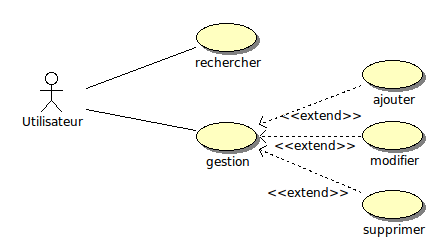
\includegraphics[scale=0.70]{images/SimpleUseCase.png}
	\captionof{figure}{Diagramme de cas d'utilisation}
\end{center}

\subsection{Requêtes}

	Notre serveur prendra en entrée une requête dont la syntaxe correspondra au langage SQL. Mais notre système ne pourra gérer toute la complexité de ce langage. Nous le limiterons donc à quelques instructions : select, insert, update, delete.\\
	De plus, et toujours dans un soucis d'efficacité, nous n'accepterons dans un premier temps, que des instructions dites basiques (toutes les instructions entre crochets sont optionnelles) :\\
- select column\_name [, column\_name2...] from table\_name [, table\_name2] [where column\_name = value...];\\
- insert into tabel\_name values(value\_table, value\_table2...) [where column\_name = value and column\_name2 = value2...];\\
- update table\_name set column\_name = value1 [, column\_name2  = value2] [where column\_name = value...];\\
- delete from table\_name [, table\_name2] [where column\_name = value...];\\
	Nous avons donc mis en place un type requête particulier :\\

\begin{center}
	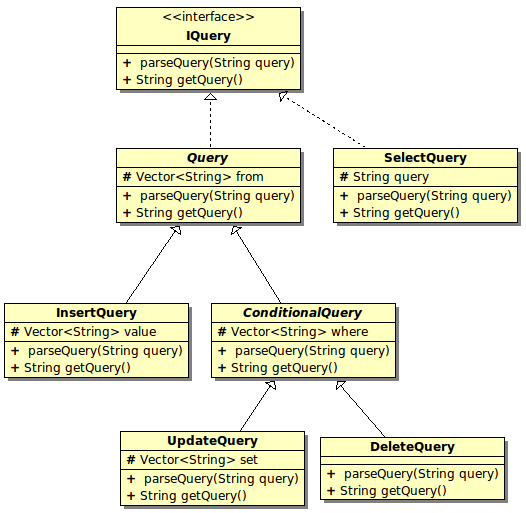
\includegraphics[scale=0.70]{images/QueryHierarchie.png}
	\captionof{figure}{Diagramme de classes : Query}
\end{center}

\subsection{Bases de données}

	Pour la distribution de nos données, nous avons décidé de partager nos données verticalement :\\
- les facteurs de transmissions d'une maladie\\
- les virus à l'origine d'une maladie\\
- le nom des maladies\\
- le nombre de cas recensés d'une maladie par zone, cette base de donnée sera une base virtuelle et sera donc découpée horizontalement par zone OMS (ici nous en prendrons trois : ???????, ???????, ???????)\\
	Ce qui donne le shéma de tables suivant :\\

\subsection{Dérivation puis Intégration}

	Maintenant que nous avons réparties nos données sur différents SGBD avec une approche dite de dérivation. Nous devons nous demander comment allons nous rendre possible la recherche sur ces différentes bases. Deux méthodes s'offrent à nous : nous continuons à dériver, ou nous intégrons nos différents schémas de bases.\\
	La première solution revient à découper notre schéma global de façon à ce qu'il colle à nos schémas locaux : donc à chaque base de données. Cette solution est la plus simple des deux mais nécessite de gros efforts d'implémentation puisque le schéma global doit être découpé en schémas locaux "à la main" pour chaque base de données. De plus cette solution devient inmaintenable lors du changement de schémas de base : en d'autres termes il faut se replonger dans la programmation.\\
	La deuxième revient à prendre tous les schémas locaux pour faire émerger un schéma global. Cette solution est bien plus compliquée au niveau de la réflexion et de la logique qu'il y a derrière. Mais la généricité de l'implémentation permet de perdre moins de temps en cas de changement des schémas des bases de données. En effet nous avons imaginé une solution entièrement basée sur les méta-tables, ce qui nous permet d'abstraire tout notre code afin de le rendre réutilisable et modulable. Nous avons donc en toute logique retenu cette deuxième solution.\\

\begin{center}
	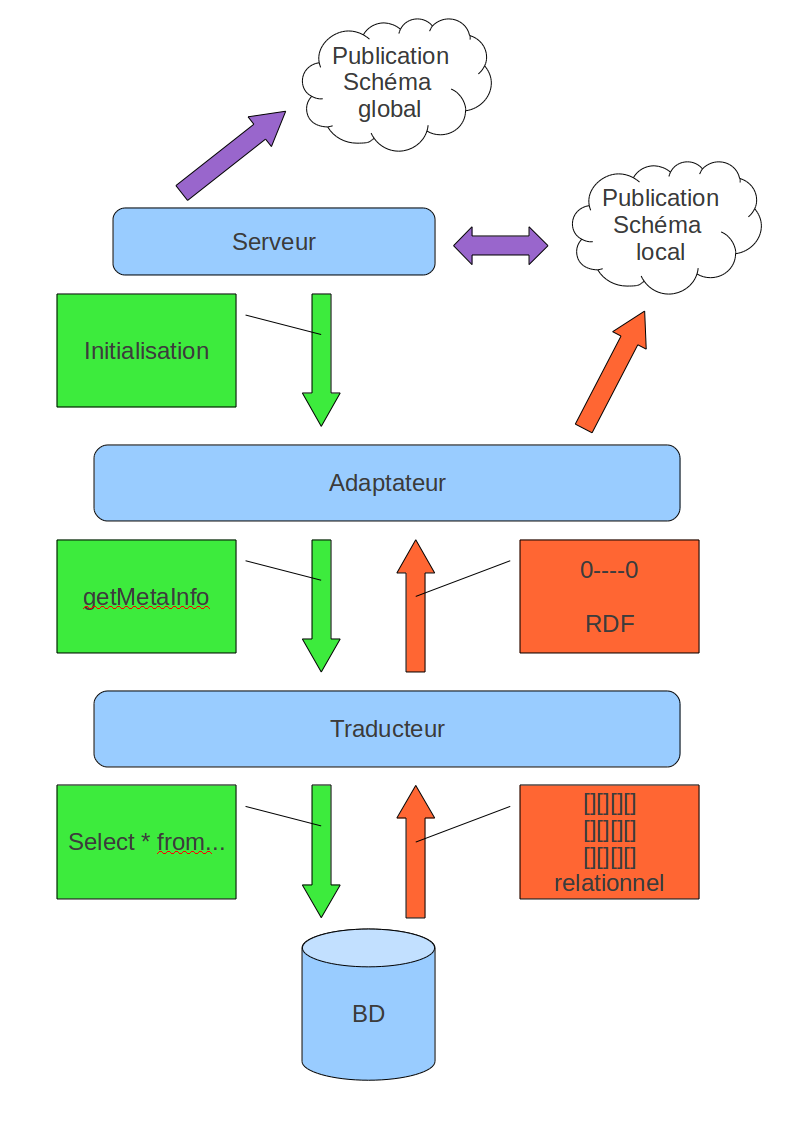
\includegraphics[scale=0.50]{images/initialisationSysteme.png}
	\captionof{figure}{Schéma d'initialisation serveur}
\end{center}

\subsection{Intégration}
	
	Puisque notre système repose sur les méta-informations des schémas locaux, le problème suivant est de pouvoir les rassembler pour faire émerger un schéma global correspondant à toutes les informations accessibles par un utilisateur.\\
	Pour réaliser cela nous avons immédiatement choisi la technologie RDF. En effet elle nous permet de représenter nos données sous forme de triplets : deux entités et une relation entre eux. Ce système nous permet d'ajouter à volonté des relations de tous types entre toutes nos entités. Vous comprendrez donc qu'il devient facile de regrouper des entités de différentes bases de données pour faire émerger notre fameux schéma global, en précisant que les données d'une base sont équivalentes au même données d'une autre.\\
	De plus RDF nous est fourni avec plusieurs outils très utiles :\\
	- D2RQ : traducteur d'objet relationnel en objet rdf.
	- N3 : cette notation qui va de paire avec D2RQ permet de lier des bases de données avec des objets rdf. En décrivant le mappage entre les tables et colonnes d'un côté et les types RDF de l'autre, D2RQ peut construire tout le schéma RDF correspondant à une base de données. Nous utiliserons donc D2RQ comme traducteur pour toutes nos bases de données.\\
	- SparQL : ce langage permet de réaliser très simplement des requêtes complexes dans nos triplets RDF. Et notamment de faire émerger des connaissances plus subtilement que par des recherches "classiques" basées sur la comparaison de valeurs.\\
	Le seul problème de D2RQ est qu'il permet de faire tout ce travail qu'en sélection. En effet nous ne pouvons pas insérer, mettre à jour ou supprimer des données d'une base. Il faudra donc trouver un autre moyen.\\
	Nous nous servirons donc de RDF aussi bien pour réaliser les requêtes de sélection de nos utilisateurs, que pour diriger nos requêtes vers telle ou telle base de données en fonction des schémas locaux.\\

\subsubsection{Schéma ontologique des Maladies de leur transmission et de leur facteur}

\begin{center}
	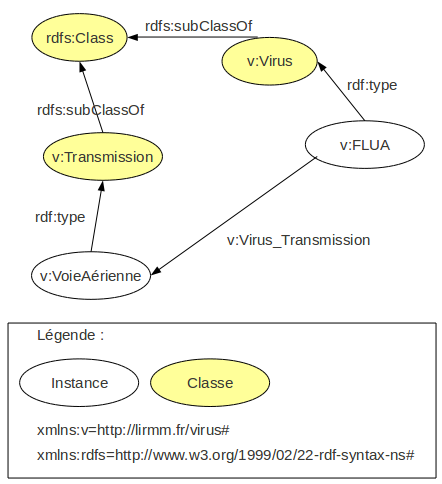
\includegraphics[scale=0.70]{../rdf/rdf-virusTransmission.png}
	\captionof{figure}{Schéma RDF MaladiesTransmission}
\end{center}

\begin{center}
	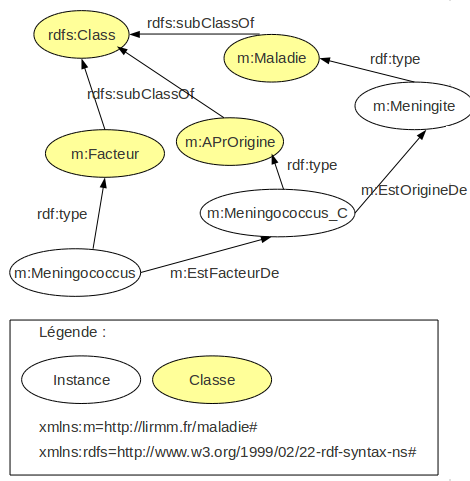
\includegraphics[scale=0.70]{../rdf/rdf-MaladieFacteur.png}
	\captionof{figure}{Schéma RDF MaladieFacteurs}
\end{center}

\begin{center}
	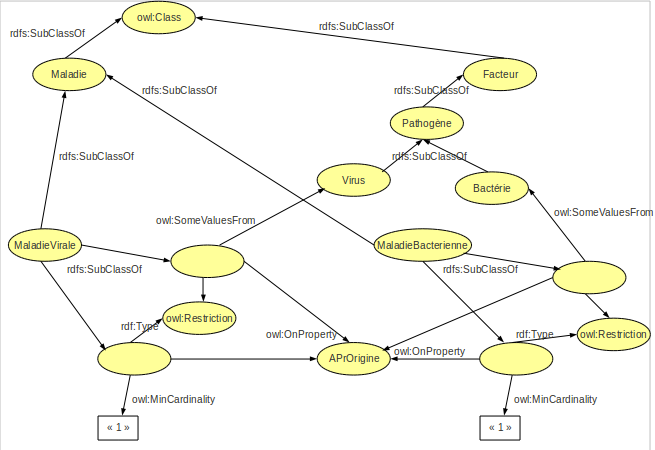
\includegraphics[scale=0.70]{../rdf/rdf-schemaMaladie.png}
	\captionof{figure}{Schéma ontologique Maladie}
\end{center}

\subsubsection{Schéma RDF CIM}

\subsubsection{Schéma RDF Recencement}

\subsubsection{Schéma RDF Global}

\subsection{Insertion, Modification et Suppression}
	
	Le dernier problème restant est donc de savoir comment nous allons insérer, modifier ou supprimer nos données des bases. Pour cela nous utiliserons la technique classique des traducteurs. Il y aura donc un traducteur par SGBD différent afin de faire correspondre la requête entrante aux normes de la base de données.

\newpage

\section{Modèle de conception}

\begin{center}
	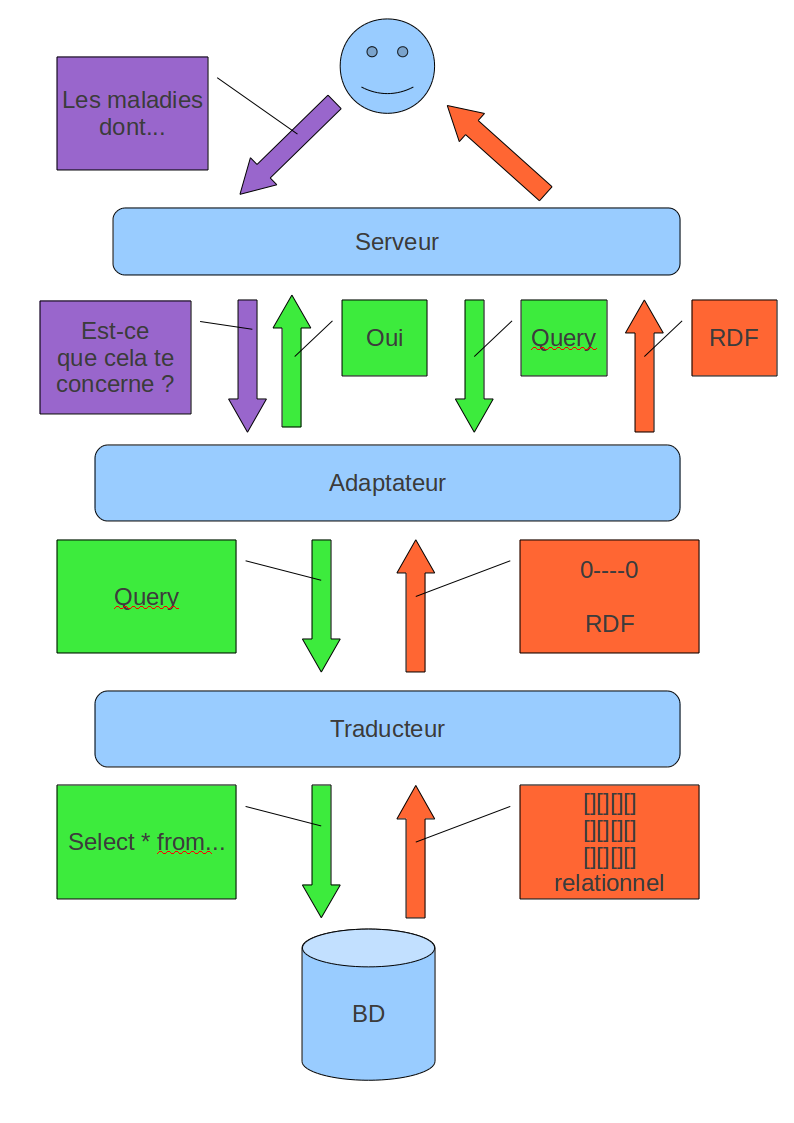
\includegraphics[scale=0.50]{images/selectQuerySysteme.png}
	\captionof{figure}{Schéma de requête}
\end{center}

\subsection{Serveur pseudos-médiateurs}

	Comme nous pouvons le voir sur ce schéma, le serveur sera le premier maillon de la chaine à recevoir la requête de l'utilisateur. Il aura alors la charge de transformer la requête qui arrive sous forme de chaine de caractères en type Query. Pour cela nous mettrons en place une fabrique à Query. Ensuite le serveur demandera à l'adapteur principal si la requête le concerne, si c'est le cas il lui transmettra la partie de la requête qui lui correspond.\\
	Il n'aura plus alors qu'à attendre le résultat, qui lui sera retourné par l'adaptateur, et au besoin transformer celui-ci du format rdf au format souhaité.\\
	Puisque notre serveur est au centre de la recherche : il prend la recherche et retourne le résultat, nous avons décidé de le caractériser par le nom pseudo-médiateur. En effet dans une architecture classique le médiateur est celui qui fractionne les requêtes pour que celles-ci correspondent au schéma local des adaptateurs. C'est ce que fait notre serveur, mais un médiateur au sens propre du terme, à d'autres exsigences que nous ne traiterons pas dans ce projet, d'où le nom de pseudo-médiateur.

\subsection{Adaptateurs}

	Nos adaptateurs sont les pièces principales du projet. Ils devront publier le schéma local des bases de données dont ils ont la responsabilité. Ces schémas seront sous la forme RDF pour faciliter la recherche. Ils contiendront le noms des tables et des colonnes des bases.\\
	Pour faciliter l'implémentation nous avons immaginé deux types d'adaptateur : les composites et les finaux.
	Les adaptateurs composites, sont des adaptateurs qui ont à leur charge non pas une base de données mais des adaptateurs qui peuvent être eux aussi composites ou finaux. Ces adaptateurs devront donc pouvoir faire émerger un schéma rassemblant l'ensemble de leur sous-adaptateurs.\\
	Puisqu'un adaptateur permet de faire tout cela, nous avons décidé d'utiliser un adaptateur composite dans notre serveur. Celui-ci devra alors faire émerger le schéma global de nos bases de données.

\subsection{Traducteurs}

	Comme son nom l'indique un traducteur permet tout simplement de convertir une requête de notre système en requête compréhensible pour le SGBD. Dans le cas de la sélection nous utiliserons D2RQ comme traducteur. Pour tout le reste nous l'implémenterons nous même.

\subsection{Diagramme de classes}

\section{Implémentation}

\subsection{Initialisation}

Lorsque le serveur est instancié il charge le fichier de configuration en xml et créer un adaptateur composite. Celui-ci va chercher dans le config file les informations nécessaires à la mise en place des sous-adaptateurs. Chaque adaptateur composite devra avoir un fichier owl pour lui signifier l'ontologie permettant de créer le schéma global. Ce fichier ne devra comporter que les points de liaisons des divers schémas locaux. Il construira alors les sous-adaptateurs.

Lorsque l'adapteur est terminal un fichier N3 lui sera alors fourni pour qu'il puisse construire son traducteur. De plus il devra avoir la configuration nécessaire à la création d'une DataBase. Il pourra donc utiliser la fabrique pour créer le bon traducteur.

\subsection{Requête}

Lorsque tout est initalisé le serveur rentre dans sa boucle run(), cette méthode doit appeler successivement interface.read() et afficher le résultat en appellant interface.write(). 

Lorsqu'une requête arrive le serveur doit construire une IQuery à l'aide de la fabrique. Il n'a enssuite qu'à appeler mediatorLike.exec(). Celui-ci va appeler sur tous ces sous-adaptateurs isQueryMatching() et si c'est vrai il appellera alors exec(). Lorsqu'un traducteur final sera appelé il passera la requête à son traducteur par le biais de la fonction exec(). Celui-ci devra tout d'abord vérifier de quel type est la requête, si elle de type select le traducteur N3 sera appelé sinon ce sera la fonction abstraite, qui aboutira dans le bon traducteur correspondant au bon sgbd.

Lorsque le résultat de la requête sera retournée à l'adaptateur-composite celui-ci devra ajouter à son modèle ontologique les triplets récupérés (toujours dans le cas où c'est un select). En remontant toute la hiérarchie notr emodèle ontologique global se construira. Et ainsi nous retournerons le résultat de la requête à l'utilisateur.

\subsection{Inconvénients}

Si l'utilisateur ne fait une recherche que sur une partie des adaptateurs, il récupèrera le schéma ontologique global du système.

\subsection{XML de configuration}

<raja>
	<CompositeAdapter><!-- Adaptateur général : contenant le schéma global -->
		<OWL url="" />
		<CompositeAdapter><!-- Adaptateur MaladieVirus -->
			<OWL url="" />
			<CompositeAdapter><!-- Adaptateur Maladie -->
				<OWL url="" />
				<TerminalAdapter><!-- Traducteur ???? -->
					<Traducteur>Vertical</Traducteur>
					<N3 url="" />
					<Database>
						<dataBaseName></dataBaseName>
						<address></address>
						<userName></userName>
						<port></port>
						<password></password>
					</Database>
				</TerminalAdapter>
			</CompositeAdapter>
			<CompositeAdapter><!-- Adaptateur Virus -->
				<OWL url="" />
				<TerminalAdapter><!-- Traducteur ???? -->
					<Traducteur>Vertical</Traducteur>
					<N3 url="" />
					<Database>
						<dataBaseName></dataBaseName>
						<address></address>
						<userName></userName>
						<port></port>
						<password></password>
					</Database>
				</TerminalAdapter>
			</CompositeAdapter>
		</CompositeAdapter>
		<CompositeAdapter><!-- Adaptateur Recenssement -->
			<OWL url="" />
			<TerminalAdapter><!-- Traducteur ???? -->
				<Traducteur>Horizontal</Traducteur>
				<N3 url="" />
				<Database>
					<dataBaseName></dataBaseName>
					<address></address>
					<userName></userName>
					<port></port>
					<password></password>
				</Database>
			</TerminalAdapter>
		</CompositeAdapter>
	</CompositeAdapter>
</raja>

\subsection{Fabrique}

\subsubsection{Requête}

\subsubsection{Traducteur}

\begin{center}
	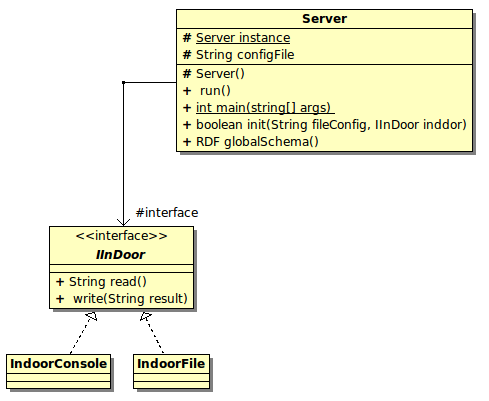
\includegraphics[scale=0.75]{images/Serveur.png}
	\captionof{figure}{Diagramme de classe du serveur}
\end{center}

\newpage

\section{Glossaire}

	\begin{itemize}
		\item \textbf{SGBD} : Système de gestion de bases de données.\\
		\item \textbf{schéma global} : le schéma de nos tables et de nos colonnes comme s'il ne s'agissait que d'une seule base de données.\\
		\item \textbf{schéma local} : le schéma physiquement stoqué sur une base de donnée particulière.\\
		\item \textbf{méta-informations} : les informations concernant le nom des tables et des colonnes d'une base de donnée.\\
		\item \textbf{requête} : dans notre système nous parlons de deux sortes de requêtes différentes, les requêtes du client donc qui arrivent dans notre serveur sous forme de chaine de caractères et les requêtes internes qui sont ces même requêtes mais transformées en objet.\\
	\end{itemize}
\newpage
\section{Annexes}

\subsection{Schéma des tables des bases de données}


\end{document}
